\chapter{Integrali di linea}

Vogliamo definire l'integrale di funzioni complesse su curve nel piano complesso. Per fare ciò parametriziamo le curve complesse su un intervallo reale. 

\begin{definition}
	\label{defn:integrale-funzione-complessa-parametrizzata-su-intervallo-reale}
	Sia $\morphism{f}{\left[a,b\right]\subset \R}{\C}$ una funzione continua, con $f(t) = u(t), iv(t)$ allora 
	\begin{equation*}
	\begin{aligned}
	\int_{a}^{b} f(t)\ dt := \int_{a}^{b} u(t)\ dt + i \int_{a}^{b} v(t)\ dt 
	\end{aligned}
	\end{equation*}
\end{definition}

\begin{proposition}
	\label{prop:proprieta-funzione-complessa-parametrizzata-su-intervallo-reale}
	Valgono le seguenti proprietà per l'integrale in Definizione \ref{defn:integrale-funzione-complessa-parametrizzata-su-intervallo-reale}
	\begin{enumerate}
		\item è lineare, infatti, per ogni $\lambda, \mu \in \C$ e $\morphism{f,g}{\left[a,b\right]}{\C}$ vale
		\begin{equation*}
		\begin{aligned}
		\int_{a}^{b} \lambda f(t)  + \mu g(t)\ dt = \lambda \int_{a}^{b} f(t)\ dt + \mu \int_{a}^{b} g(t)\ dt   
		\end{aligned}
		\end{equation*}
		\item commuta con l'operazione $\Re, \Im$.
		\begin{equation*}
		\begin{aligned}	
		\Re\left(\int_{a}^{b} f(t)\ dt\right) = \int_{a}^{b} \Re(f(t))\ dt \quad\ \Im\left(\int_{a}^{b} f(t)\ dt\right) = \int_{a}^{b} \Im(f(t))\ dt
		\end{aligned}
		\end{equation*} 
		\item vale la seguente disuguaglianza
		\begin{equation*}
		\begin{aligned}
		\left|\int_{a}^{b} f(t)\ dt\right| \le \int_{a}^{b} |f(t)|\ dt
		\end{aligned}
		\end{equation*}
		\item Se $\morphism{\theta}{\left[c,d\right]}{\left[a,b\right]}$ è di classe $C^1$ e ha un inversa di classe $C^1$ allora
		\begin{equation*}
		\begin{aligned}
		\int_{\theta(c)}^{\theta(d)} f(t)\ dt = \int_{a}^{b} f(\theta(t))\theta'(t)\ dt
		\end{aligned}
		\end{equation*}
	\end{enumerate} 
\end{proposition}
\begin{proof}[1]
	Il primo punto deriva dalla linearità dell'integrale di Riemann. 
	Basta dividere in parte reale e immaginaria della funzione $f = u+ iv$.
\end{proof}

\begin{proof}[2]
	Segue dalla linearità dividendo la funzione in parte reale e immaginaria.	
\end{proof}

\begin{proof}[3]
	Poniamo $\omega := \int_{a}^{b} f(t)\ dt$, allora se $\omega = 0$ è dimostrata. Se $\omega \neq 0$ allora poniamo $u = \overline{\omega}/|\omega|$, osserviamo che $|u|=1$. Da cui
	\begin{equation*}
	\begin{aligned}
	|w| = uw = \int_{a}^b \Re(uf(t))\ dt \le \int_{a}^b |uf(t))|\ dt = \int_{a}^b |f(t))|\ dt  
	\end{aligned}
	\end{equation*}
\end{proof}

\begin{proof}[4]
	Questo si può vedere come la Formula dell'area  
	\begin{equation*}
	\begin{aligned}
	\int_{\theta(a,b)} f(z) dz & = \int_{\theta(a,b)} u(x,y) \mathcal{L}^2(x,y)
	+ i\int_{\theta(a,b)} v(x,y) \mathcal{L}^2(x,y)\\
	& = \int_a^b u(\theta(t))\theta'(t) \mathcal{L}^1(t) 
	+ i\int^b_a v(\theta(t))\theta'(t) \mathcal{L}^2(t)\\
	& = \int_a^b f(\theta(t)) \theta'(t)\ dt		
	\end{aligned}
	\end{equation*}
\end{proof}

\begin{definition}
	\label{defn:curva-c1}
	Una \textbf{curva di classe $C^1$} nel piano complesso è una funzione $\morphism{\gamma}{J=\left[a,b\right]}{\C}$ di classe $C^1$. L'immagine $\gamma(J) \subset \C$ è detta \textbf{traccia o sostegno della curva}. Una curva di classe $C^1$ a tratti è una funzione continua $\morphism{\gamma}{J}{\C^1}$, di classe $C^1$ su $J$ meno un numero finito di punti.\\ 		
\end{definition}

\begin{definition}
	\label{defn:riparametrizzazione-curva-classe-c1}
	Sia $\morphism{\theta}{\left[c,d\right]}{\left[a,b\right]}$ una funzione di classe $C^1$, con inversa di classe $C^1$. Supponiamo che $\theta' > 0$ su $\left[c, d\right]$. Dunque $\theta$ è monotona crescente, con $\theta(c) = a$, $\theta(d) = b$. La curva di classe $C^1$ definita da $\morphism{\overline{\gamma}(s) = \gamma(\theta (s))}{\left[c,d\right]}{\C}$ è detta \textbf{riparametrizzazione di $\gamma$}.
\end{definition}

\begin{definition}
	\label{defn:lunghezza-di-curva-classe-c1}
	La \textbf{lunghezza} della curva di classe $C^1$ $\morphism{\gamma}{\left[a,b\right]}{\C}$ è definita come l'integrale 
	\begin{equation*}
	\begin{aligned}
	l(\gamma) := \int_{a}^{b} |\gamma'(t)|\ dt
	\end{aligned}
	\end{equation*}
\end{definition}

\begin{definition}
	\label{defn:integrale-di-linea}
	Sia $\morphism{\gamma}{\left[a,b\right]}{\C}$ una curva di classe $C^1$ con sostegno contenuto in un aperto $\Omega \subset \C$. Sia $\morphism{f}{\Omega}{\C}$ allora
	\begin{equation*}
	\begin{aligned}
	\int_\gamma f(z)\ dz := \int_{a}^b f(\gamma(t)) \gamma'(t) \ dt
	\end{aligned}
	\end{equation*}  
\end{definition}

\begin{remark}
	La definizione \ref{defn:integrale-di-linea} è dipendente dalla parametrizzazione utilizzata, ma ciò non toglie che dia, per parametrizzazioni che non cambiano l'orientazione della curva, lo stesso risultato (come si può riparametrizzando avanti e indietro la curva).
\end{remark}

\begin{proposition}
	\label{prop:proprieta-integrale-di-linea}
	L'integrale in Definizione \ref{defn:integrale-di-linea} ha le seguenti proprietà
	\begin{enumerate}
		\item è lineare, ovvero date $\morphism{f,g}{\Omega \subset \C}{\C}$ e $\lambda, \mu \in \C$ vale
		\begin{equation*}
		\begin{aligned}
		\int_{\gamma} \lambda f(z) + \mu g(z) \ dz =  \lambda \int_{\gamma} f(z) \ dz + \mu \int_{\gamma} g(z) \ dz 
		\end{aligned}
		\end{equation*}
		\item vale la seguente disequazione per ogni $\morphism{f}{\Omega}{\C}$
		\begin{equation*}
		\begin{aligned}
		\left|\int_{\gamma} f(z) \ dz\right| \le \max_{\gamma} |f(z)| \mathcal{H}^1(\gamma)	
		\end{aligned}
		\end{equation*}
		\item sia $-\gamma(t) := \gamma(a+b-t)$ la curva percorsa in senso opposto a quello di $\gamma$, allora
		\begin{equation*}
		\begin{aligned}
		\int_{-\gamma} f(z) \ dz = - \int_{\gamma} f(z) \ dz
		\end{aligned}
		\end{equation*}
		\item Se esiste $F$ olomorfa tale che $F' = f$ su tutto $\Omega$ allora
		\begin{equation*}
		\begin{aligned}
		\int_\gamma f(z) \ dz = F(\gamma(b)) - F(\gamma(a))
		\end{aligned}
		\end{equation*}
		In particolare, se $\gamma$ è chiusa, vale $\int_\gamma f(z)\ dz = 0$.
	\end{enumerate}
\end{proposition}
\begin{proof}[1]
	Deriva immediatamente dal punto 1 della Proposizione \ref{prop:proprieta-funzione-complessa-parametrizzata-su-intervallo-reale}.
\end{proof}
\begin{proof}[2]	
	Segue dal punto $3$ della Proposizione \ref{prop:proprieta-funzione-complessa-parametrizzata-su-intervallo-reale}:
	\begin{equation*}
	\begin{aligned}
	\left|\int_\gamma f(z)\ dz\right| \le \int^b_a |f(\gamma(t))||\gamma'(t)| \ dt \le \max_{\gamma} f(z) \mathcal{H}^1(\gamma(\left[a,b\right])) 
	\end{aligned}
	\end{equation*}
\end{proof}
\begin{proof}[3]
	È conseguenza della formula $4$ della Proposizione \ref{prop:proprieta-funzione-complessa-parametrizzata-su-intervallo-reale}. Ponendo $s = \theta(t) = a + b - t$ si ottiene
	\begin{equation*}
	\begin{aligned}
	\int_{-\gamma} f(z)\ dz = \int_{\gamma(\theta))} f(z)\ dz = -\int_{\gamma} f(z)\ dz
	\end{aligned}
	\end{equation*}
\end{proof}
\begin{proof}[4]
	Osserviamo che $\odv{F \circ \gamma}{t} = (f \circ \gamma) \gamma'$. Per cui dal teorema fondamentale del calcolo integrale
	\begin{equation*}
	\begin{aligned}
	\int^b_a f(\gamma(t))\gamma'(t)\ dt = \int_a^b (F \circ \gamma)'(t)\ dt = F(\gamma(b)) - F(\gamma(a))
	\end{aligned}
	\end{equation*}
\end{proof}

\begin{remark}
	Le stesse proprietà valgono con opportuni accorgimenti anche per curve $C^1$ quasi ovunque. Infatti basta togliere i punti in cui non è definita la curva e considerare i tratti $C^1$. 
\end{remark}

\begin{theorem}
	Non esiste una funzione logaritmo olomorfa su tutto $\C \setminus \{0\}$.
\end{theorem}
\begin{proof}
	Osserviamo che se $\gamma(t) = e^{it} \colon \left[0,2\pi\right] \to \C$ allora $\gamma'(t) = ie^{it}$. Per cui
	\begin{equation*}
	\begin{aligned}
	\int_\gamma \frac{1}{z}\ dz = \int_{0}^{2\pi} \frac{1}{e^{it}} ie^{it}\ dt = 2i\pi
	\end{aligned}
	\end{equation*}
	
	Supponiamo esista $\morphism{f}{\C \setminus \{0\}}{\C}$ funzione logaritmo olomorfa su tutto il suo dominio. Allora $e^{f(z)} = z$ e quindi si avrebbe
	\begin{equation*}
	\begin{aligned}
	1 = z' =(e^{f(z)})' = e^{f(z)} f'(z) 
	\end{aligned}
	\end{equation*}
	ovvero $f'(z) = 1/z$. Quindi $f$ sarebbe una primitiva olomorfa di $1/z$. Quindi per il punto $4$ della Proposizione \ref{prop:proprieta-integrale-di-linea} si avrebbe che $\int_{\gamma} 1/z \ dz = 0$, contraddicendo l'osservazione fatta all'inizio. 
\end{proof}

\begin{theorem}[di Goursat]
	\label{thr:groursat}
	Sia $\Omega \subset \C$ un aperto, sia $f \in \mathcal{O}(\Omega)$ e sia $R$ un rettangolo tale che $R \subset \Omega$. Allora 
	\begin{equation*}
	\begin{aligned}
	\int_{\partial R} f(z)\ dz = 0
	\end{aligned}
	\end{equation*}
	ove $\partial R$ è il bordo del rettangolo (il perimetro) percorso in senso anti-orario.
\end{theorem}
\begin{proof}
	Per ogni rettangolo $R' \subset \Omega$ definiamo 
	\begin{equation*}
	\begin{aligned}
	\eta(R') := \left| \int_{\partial R'} f(z)\ dz\right|
	\end{aligned}
	\end{equation*}
	Per cui suddividiamo $R$ in quattro sottrettangoli, $R_1, \dots, R_4$. La somma dell'intergale sul bordo dei 4 rettangoli dà l'integrale di $f$ lungo $R$ dato che i lati interni vengono percorsi in senso opposto e quindi valgono $0$. \\
	In particolare ci sarà un rettangolo $R_{i_0}$ tale che 
	\begin{equation*}
	\begin{aligned}	
	\eta(R_{i_0}) \ge \frac{\eta(R)}{4} 
	\end{aligned}
	\end{equation*}
	Suddividiamo ancora una volta $R_{i_0}$ in altri $4$ rettangoli, da cui si ottiene che esiste un rettangolo $R_{i_1} \subset R_{i_0}$ tale che 
	\begin{equation*}
	\begin{aligned}
	\eta(R_{i_1}) \ge \frac{\eta(R_{i_0})}{4} \ge \frac{\eta(R)}{16} 
	\end{aligned}
	\end{equation*}
	e procedendo iterativamente si ottiene una successione di rettangoli mano a mano più piccoli e tali che 
	\begin{equation*}
	\begin{aligned}	
	\eta(R_{i_n}) \ge \frac{\eta(R)}{4^n}
	\end{aligned}
	\end{equation*}
	Sia $\{z_n\}$ una successione di punti tale che $z_n \in \R_{i_n}$. Allora questa successione è di Cauchy dato che $|z_n - z_m| \le \diam{R_{i_n}} \le \diam{R}/2^m$ dove $m < n$. In particolare la successione converge a un certo $z^*$.\\
	Inoltre $f \in \mathcal{O}(\Omega)$ e quindi è olomorfa anche in $z^*$. Quindi essendo differenziabile in $z^*$ si ottiene che 
	\begin{equation*}
	\begin{aligned}
	|f(z) - f(z^*) - f'(z^*)(z-z^*)| < \varepsilon(z - z^*)
	\end{aligned}
	\end{equation*}
	vale per ogni $\varepsilon > 0$ e $|z - z^*| < \delta$ per qualche $\delta > 0$. Osserviamo che in particolare possiamo prendere come intorno in cui vale un rettangolo $R_{i_n}$ per $n$ ``abbastanza grande''. Per cui
	\begin{equation*}
	\begin{aligned}
	\eta(R_{i_n}) = \left|\int_{\partial R_n} f(z)\ dz\right| = 0 % TODO non so bene come scriverlo, essenzialmente e' a causa della differenziabilità che di da che è uguale a un polinomio, quindi ha primitiva e quindi va a 0
	\end{aligned}
	\end{equation*}
	da cui 
	\begin{equation*}
	\begin{aligned}
	\eta(R_{i_n}) \le \varepsilon \diam{R_{i_n}} \mathcal{H}^1(\partial R_{i_n}) \le \varepsilon \frac{K}{4^n} 
	\end{aligned}
	\end{equation*}
	ed essendo
	\begin{equation*}
	\begin{aligned}
	\frac{\eta(R)}{4^n} \le \eta(R_{i_n}) \le \varepsilon \frac{K}{4^n}
	\end{aligned}
	\end{equation*}
	allora $\eta(R) \le \varepsilon K$ e per l'arbitrarietà di $\varepsilon$ si ottiene la tesi.
\end{proof}

\begin{theorem}[Teorema di Cauchy]
	\label{thr:cauchy-integrale}
	Sia $\D \subset \C$ un disco aperto e $f$ olomorfa sul disco e $\gamma$ una curva chiusa con supporto $\gamma(I) \subset D$, allora 
	\begin{equation*}
	\begin{aligned}
	\int_\gamma f(z)\ dz = 0
	\end{aligned}
	\end{equation*}
\end{theorem}
\begin{proof}
	Essenzialmente grazie al teorema di Goursat se si lavora su un convesso puoi e $f$ olomorfa, allora $f$ ha una primitiva $F$. Per concludere basta vedere che essendo una curva chiusa $F(\gamma(a)) - F(\gamma(b)) = 0$. 
\end{proof}

\begin{corollary}
	Sia $D$ un disco aperto e sia $f$ olomorfa in $D$. Siano $\gamma_1, \gamma_2$ curve con gli stessi estremi aventi entrambe supporto in $D$. Allora
	\begin{equation*}
	\begin{aligned}	
	\int_{\gamma_1} f(z) \ dz = \int_{\gamma_2} f(z) \ dz
	\end{aligned}
	\end{equation*}
\end{corollary}

\begin{theorem}
	\label{thr:goursat-con-singolarità}
	Sia $f \in \mathcal{O}(\Omega \setminus \{a_1, \dots, a_n\})$ tale che
	\begin{equation*}
	\begin{aligned}
	\lim_{z\to a_i} (z-a_i)f(z) = 0
	\end{aligned}
	\end{equation*}
	per ogni $i \in \{1, \dots, n\}$ allora se $R$ è un rettangolo con bordo in $\Omega \setminus  \{a_1, \dots, a_n\}$ vale
	\begin{equation*}
	\begin{aligned}
	\int_{\partial R} f(z)\ dz = 0
	\end{aligned}
	\end{equation*}
\end{theorem}
\begin{proof}
	A meno di suddividere il rettangolo iniziale in più sotto rettangoli, possiamo supporre che $R$ contenga un solo punto di non derivabilità di $f$. Dividamo il rettangolo in $8$ sottorettangoli e un quadrato $Q$ come in figura
	\begin{figure}[h]
		\centering
		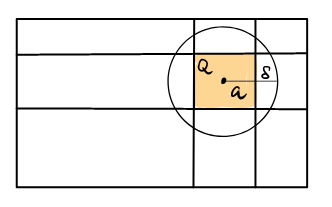
\includegraphics[width=0.4\linewidth]{./images/analisi_complessa/rectangles-singularity-integration.png}
		\caption{}
		\label{fig:rectangles-singularity-integration}
	\end{figure}
	Applicando il teorema di Goursat \ref{thr:groursat} agli otto rettangoli si ottiene che l'integrale sul bordo coincide con l'integrale sul bordo di $Q$. 
	Per ipotesi di $f$ tale che $(z-a_i)f(z) \to 0$ per $z \to a_i$, equivale a dire che per ogni $\varepsilon > 0$ esiste $\delta$ tale che se $|z - a| < \delta$ allora $f(z)(z-a) < \varepsilon$. In particolare poiché la suddivisione fatta può essere arbitraria, ovvero il lato del quadrato $Q$ possiamo sceglierlo in modo tale che per ogni $q\in Q$ vale $|q-a_i| < \delta$, per cui
	\begin{equation*}
	\begin{aligned}
	\left|\int_{\partial Q} f(z)\ dz\right| \le 4 \mathcal{H}^1(\partial Q) \max \frac{\varepsilon }{|z-a_i|} = 8\varepsilon 
	\end{aligned}
	\end{equation*}
	e per l'arbitrarietà di $\varepsilon$ segue la tesi.
\end{proof}

\begin{corollary}
	Sia $f \in \mathcal{O}(\D \setminus \{a_1, \dots, a_n\})$ tale che
	\begin{equation*}
	\begin{aligned}
	\lim_{z\to a_i} (z-a_i)f(z) = 0
	\end{aligned}
	\end{equation*}
	per ogni $i \in \{1, \dots, n\}$. Sia $\gamma$ una curva chiusa con supporto contenuto in $\D \setminus  \{a_1, \dots, a_n\}$ vale
	\begin{equation*}
	\begin{aligned}
	\int_{\gamma} f(z)\ dz = 0
	\end{aligned}
	\end{equation*}
\end{corollary}
\begin{proof}
	Si procede in maniera analoga a quanto visto per il Teorema di Cauchy \ref{thr:cauchy-integrale} per costruire una primitiva di $f$, denotiamola $F$ (questo è possibile grazie al Teorema \ref{thr:goursat-con-singolarità}). Utilizzando le curve opportune (ovvero quelle soddisfacenti le ipotesi), si ottiene la tesi.
\end{proof}
